\section{Anexes}

\begin{figure}[htbp]
    \center
    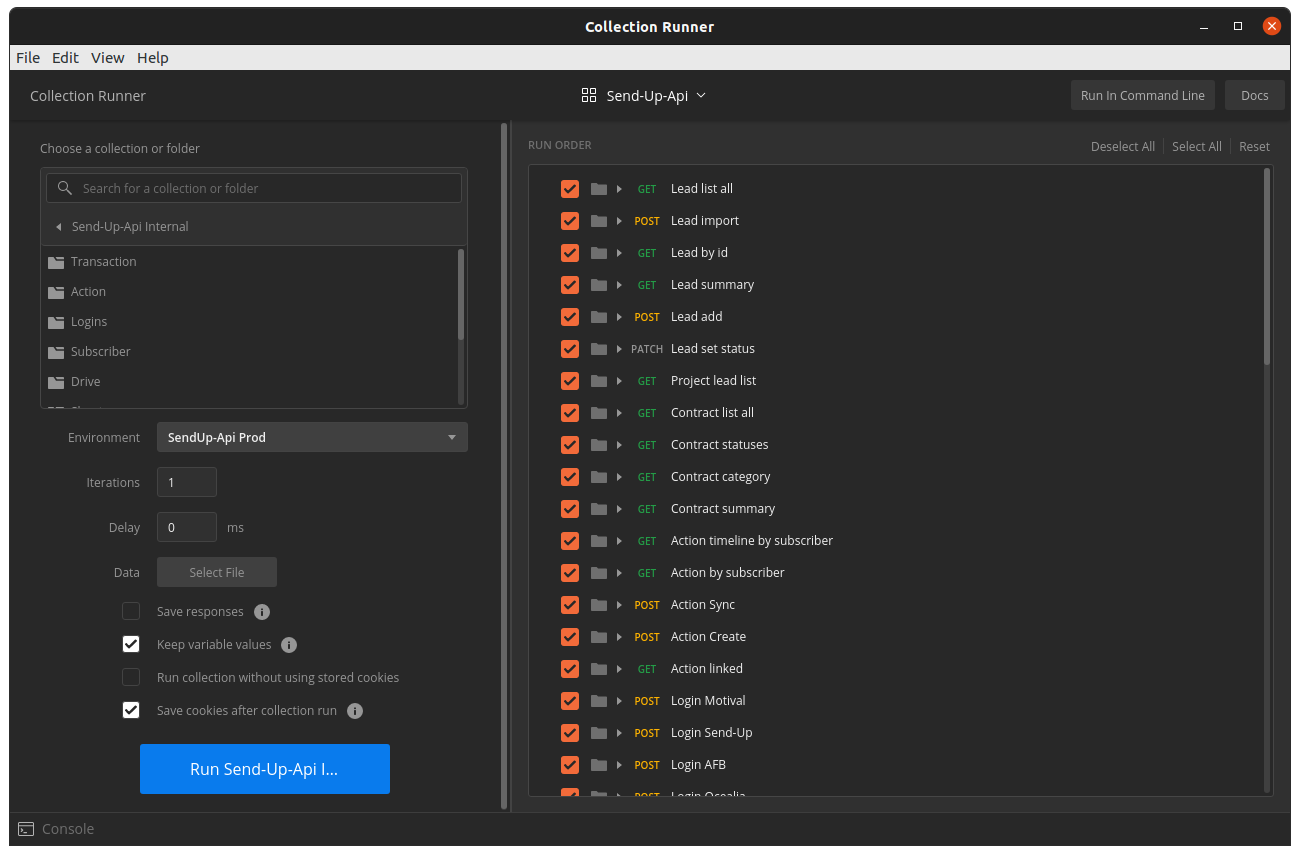
\includegraphics[width=\textwidth]{postman_collectionRunner.png}
    \caption{Exemple de collection runner Postman}
    \label{fig:postman_collectionRunner}
\end{figure}

\begin{figure}[htbp]
    \center
    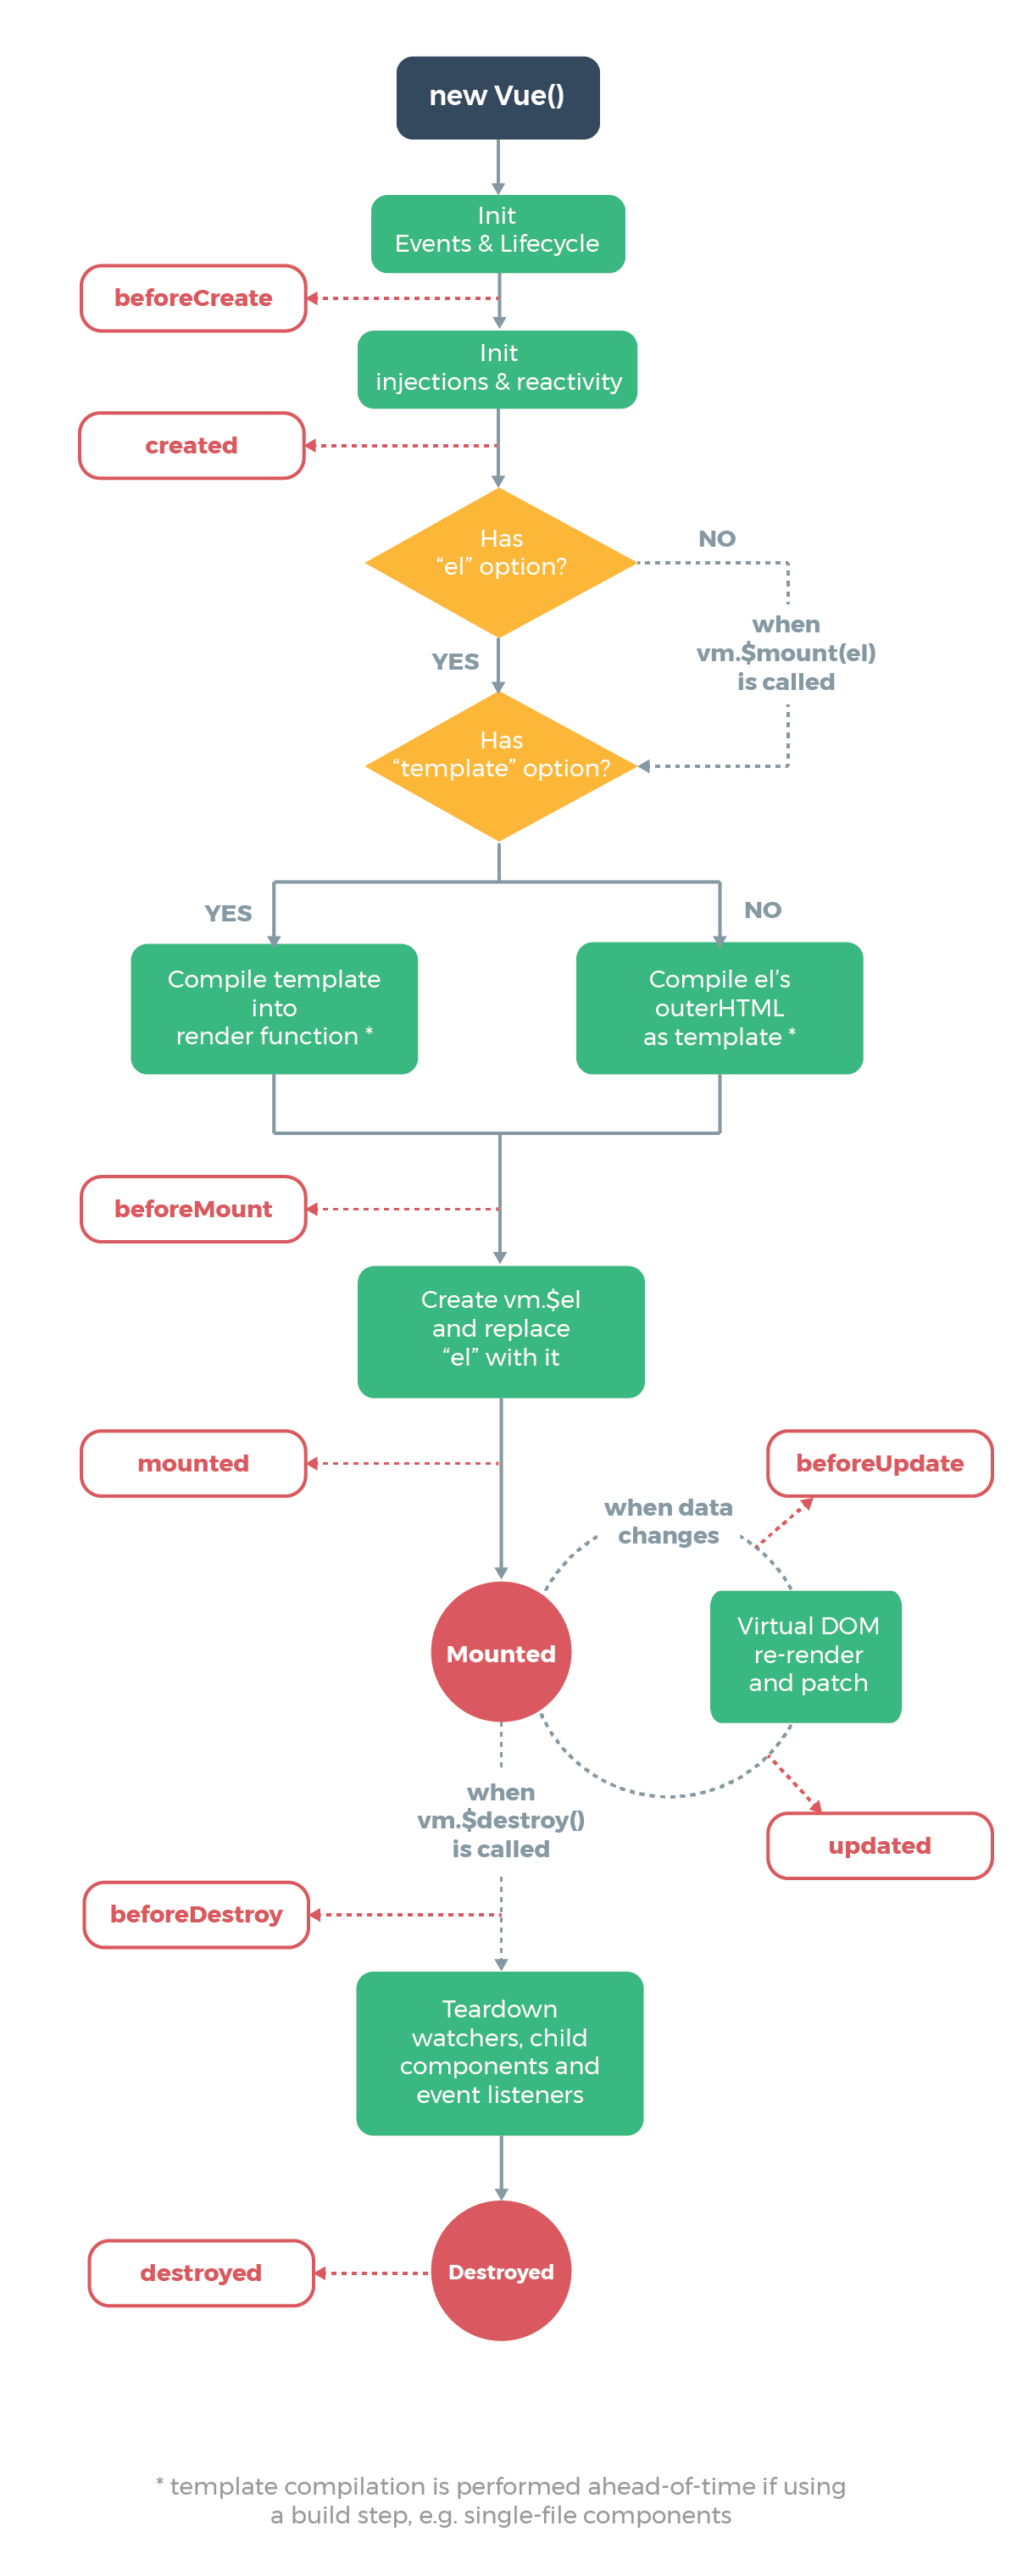
\includegraphics[width=0.5\textwidth]{vue_cycle.png}
    \caption{Schéma du cycle de vie - d'un composant vue\cite{vuelifecycle}}
    \label{fig:vue_cycle}
\end{figure}
    
\begin{figure}[htbp]
    \center 
    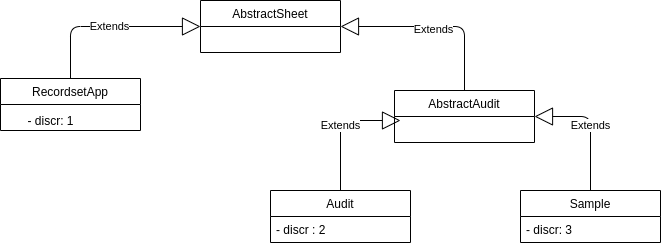
\includegraphics[width=\textwidth]{recordset.png}
    \label{fig:recordset}
    \caption{Architecture des recordset}
\end{figure}
\begin{figure}[htbp]
    \center 
    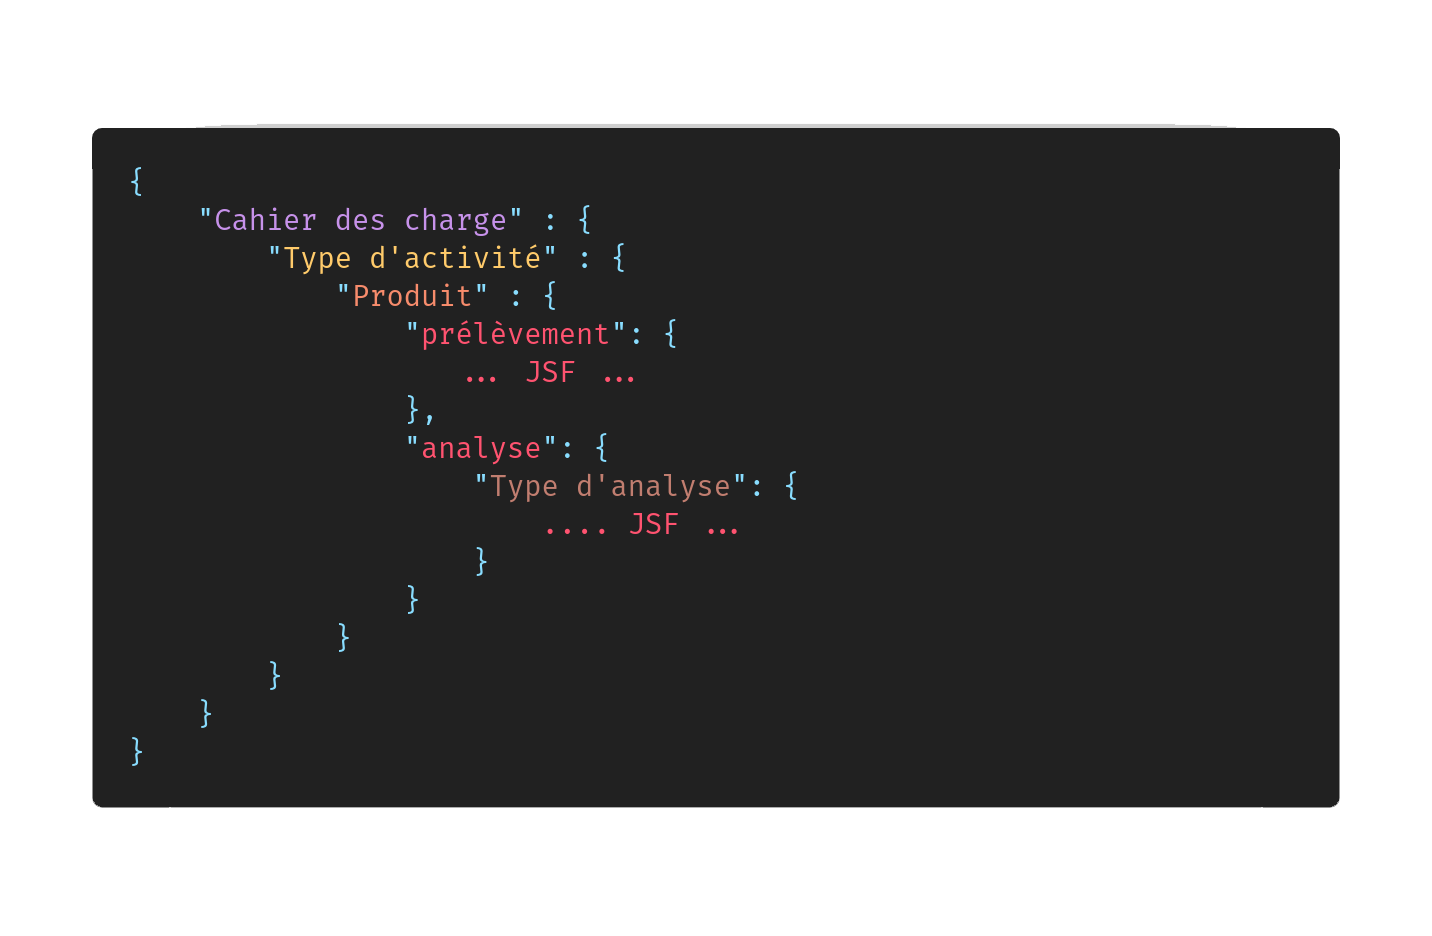
\includegraphics[width=\textwidth]{jsf.png}
    \caption{Architecture du schema JSON}
    \label{fig:jsf}
\end{figure}


\begin{figure}[htbp]
    \center 
    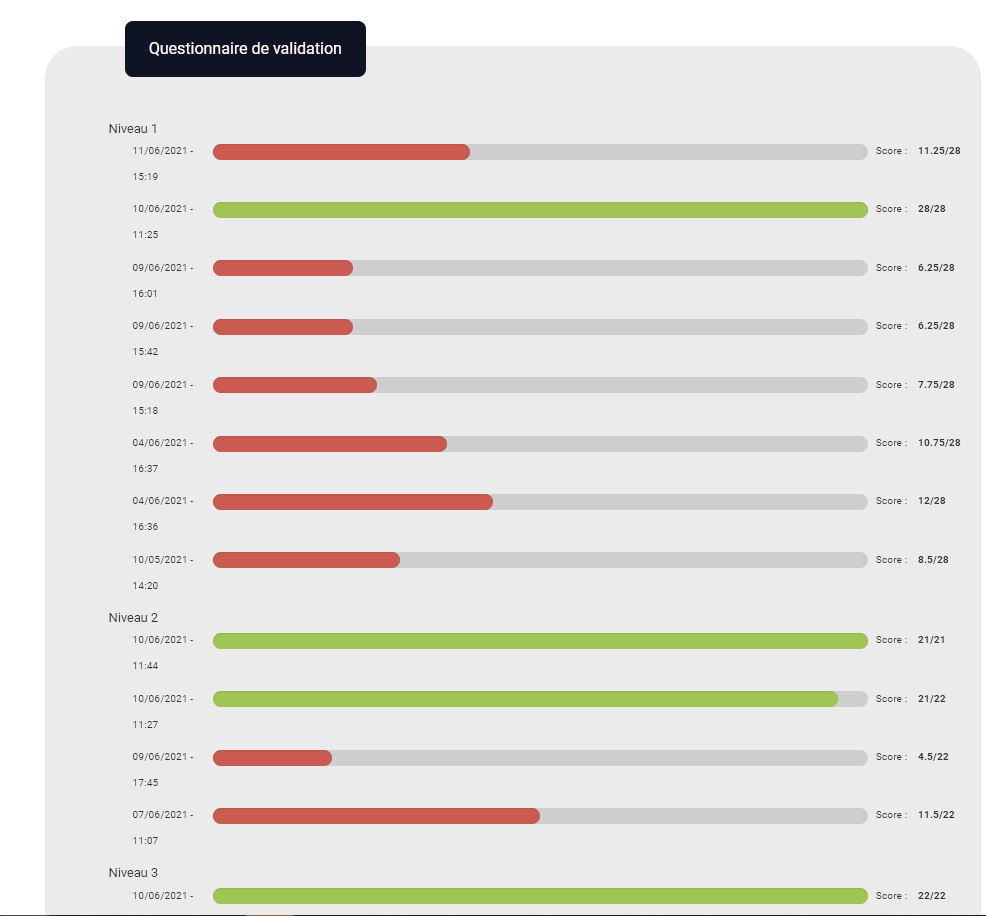
\includegraphics[width=\textwidth]{stat.png}
    \caption{Statistiques indiviuelles}
    \label{fig:statindi}
\end{figure}

\begin{figure}[htbp]
    \center 
    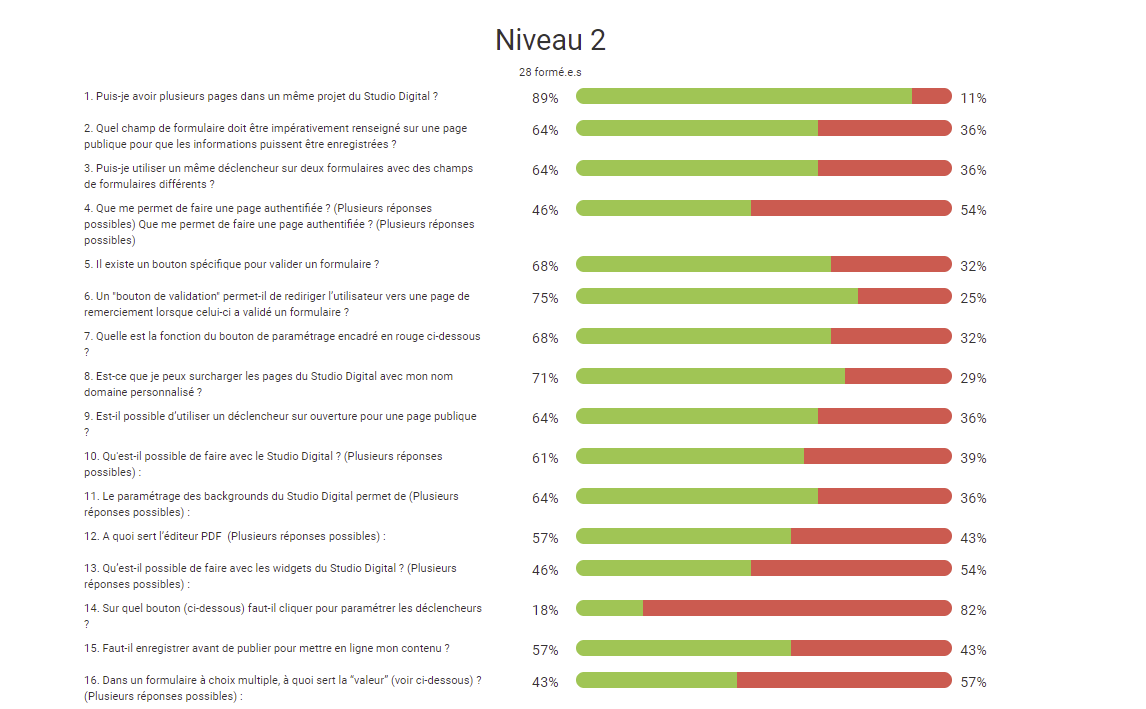
\includegraphics[width=\textwidth]{statglobal.png}
    \caption{Statistiques globales}
    \label{fig:statglobal}
\end{figure}

\begin{figure}[htbp]
    \center 
    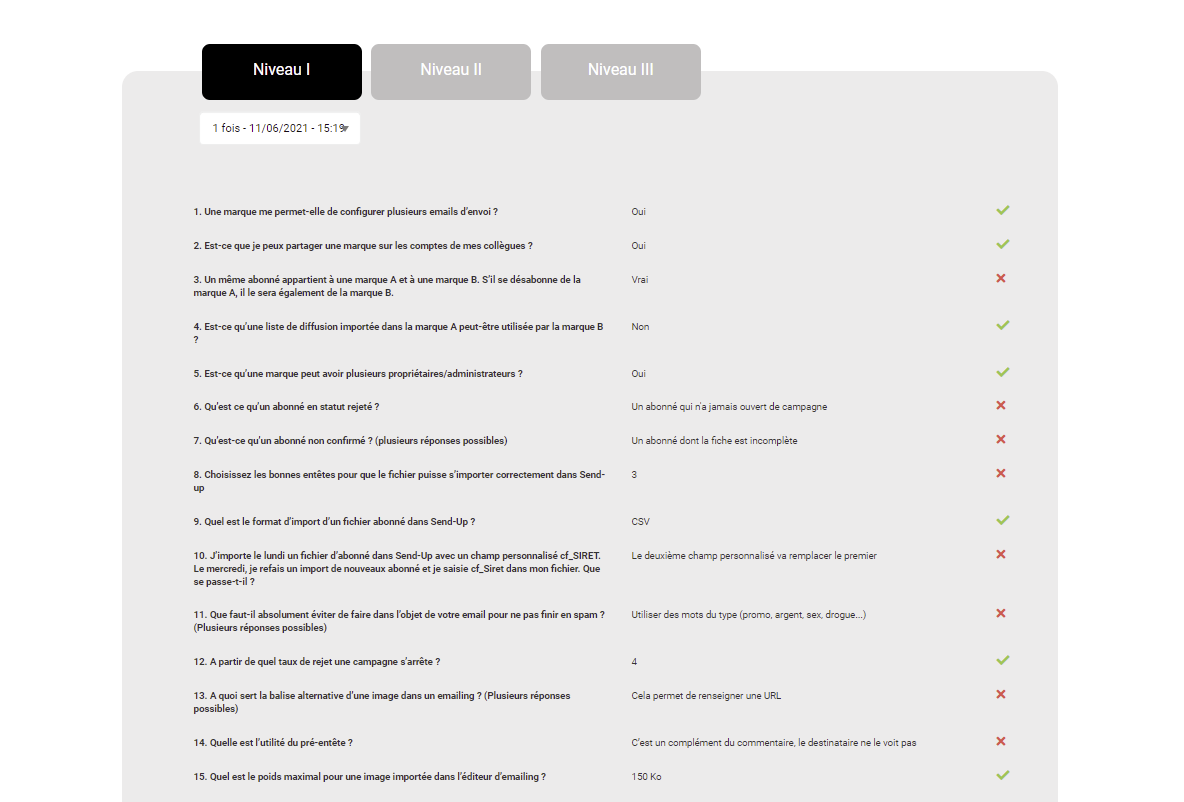
\includegraphics[width=\textwidth]{answer.png}
    \caption{Réponses au questionnaires}
    \label{fig:answer}
\end{figure}

\begin{figure}[htbp]
    \center 
    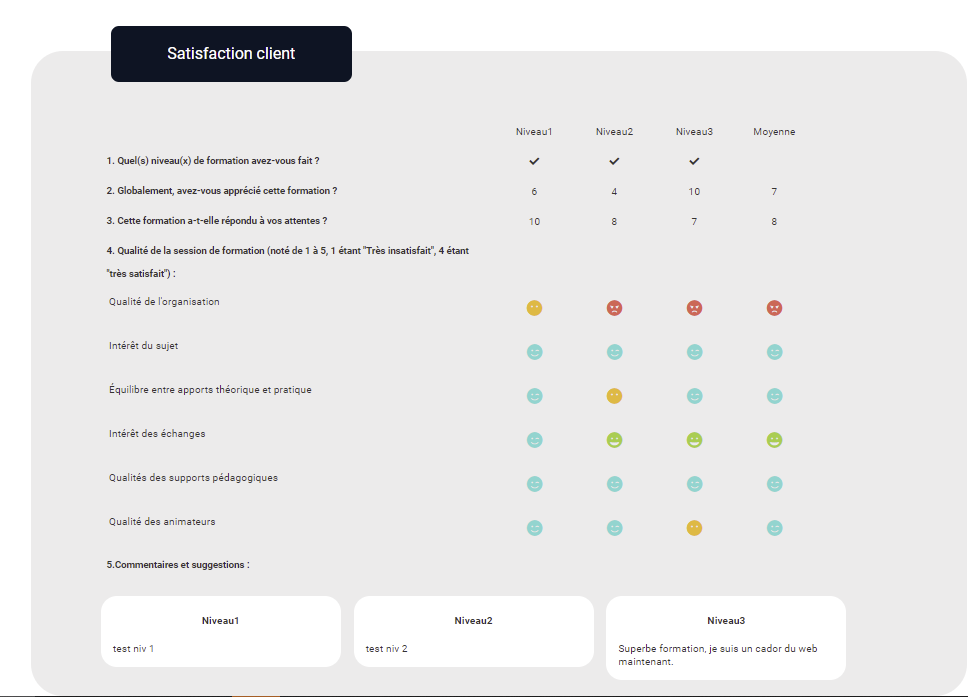
\includegraphics[width=\textwidth]{satif.png}
    \caption{Questionnaires de satisfaction}
    \label{fig:satisfaction}
\end{figure}

\begin{figure}[htbp]
    \center 
    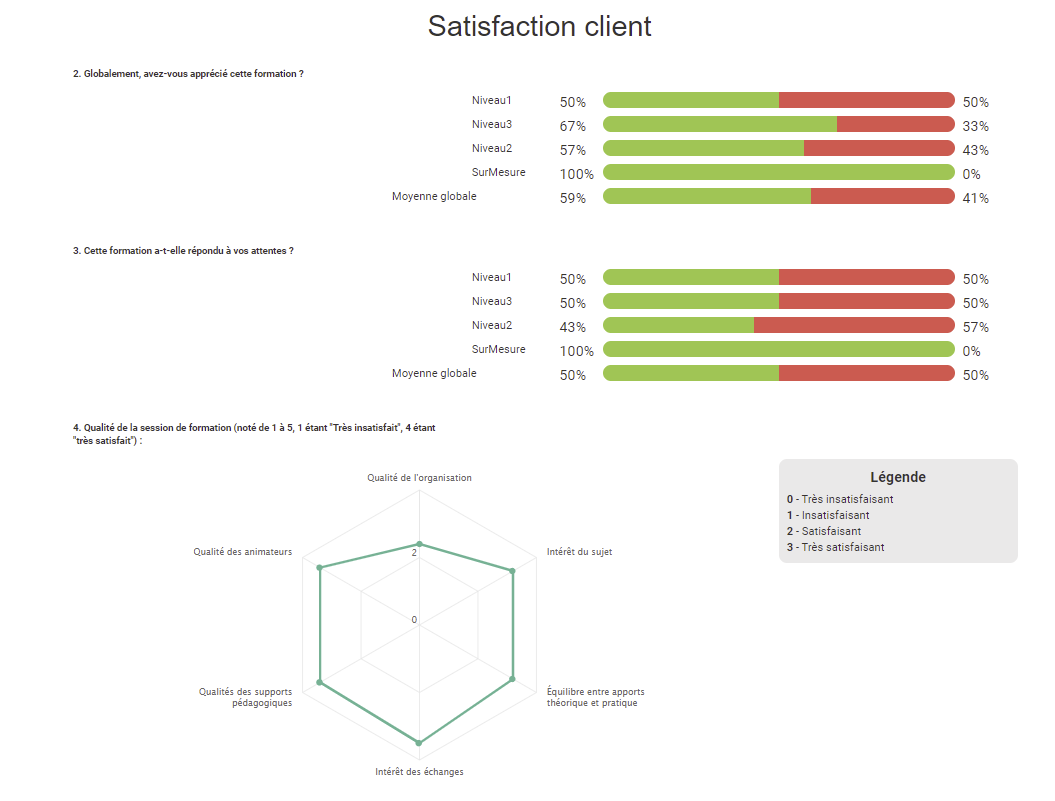
\includegraphics[width=\textwidth]{statsatif.png}
    \caption{Statistiques du questionnaire de satisfaction}
    \label{fig:satisfactionStat}
\end{figure}


\begin{figure}[htbp]
    \center 
    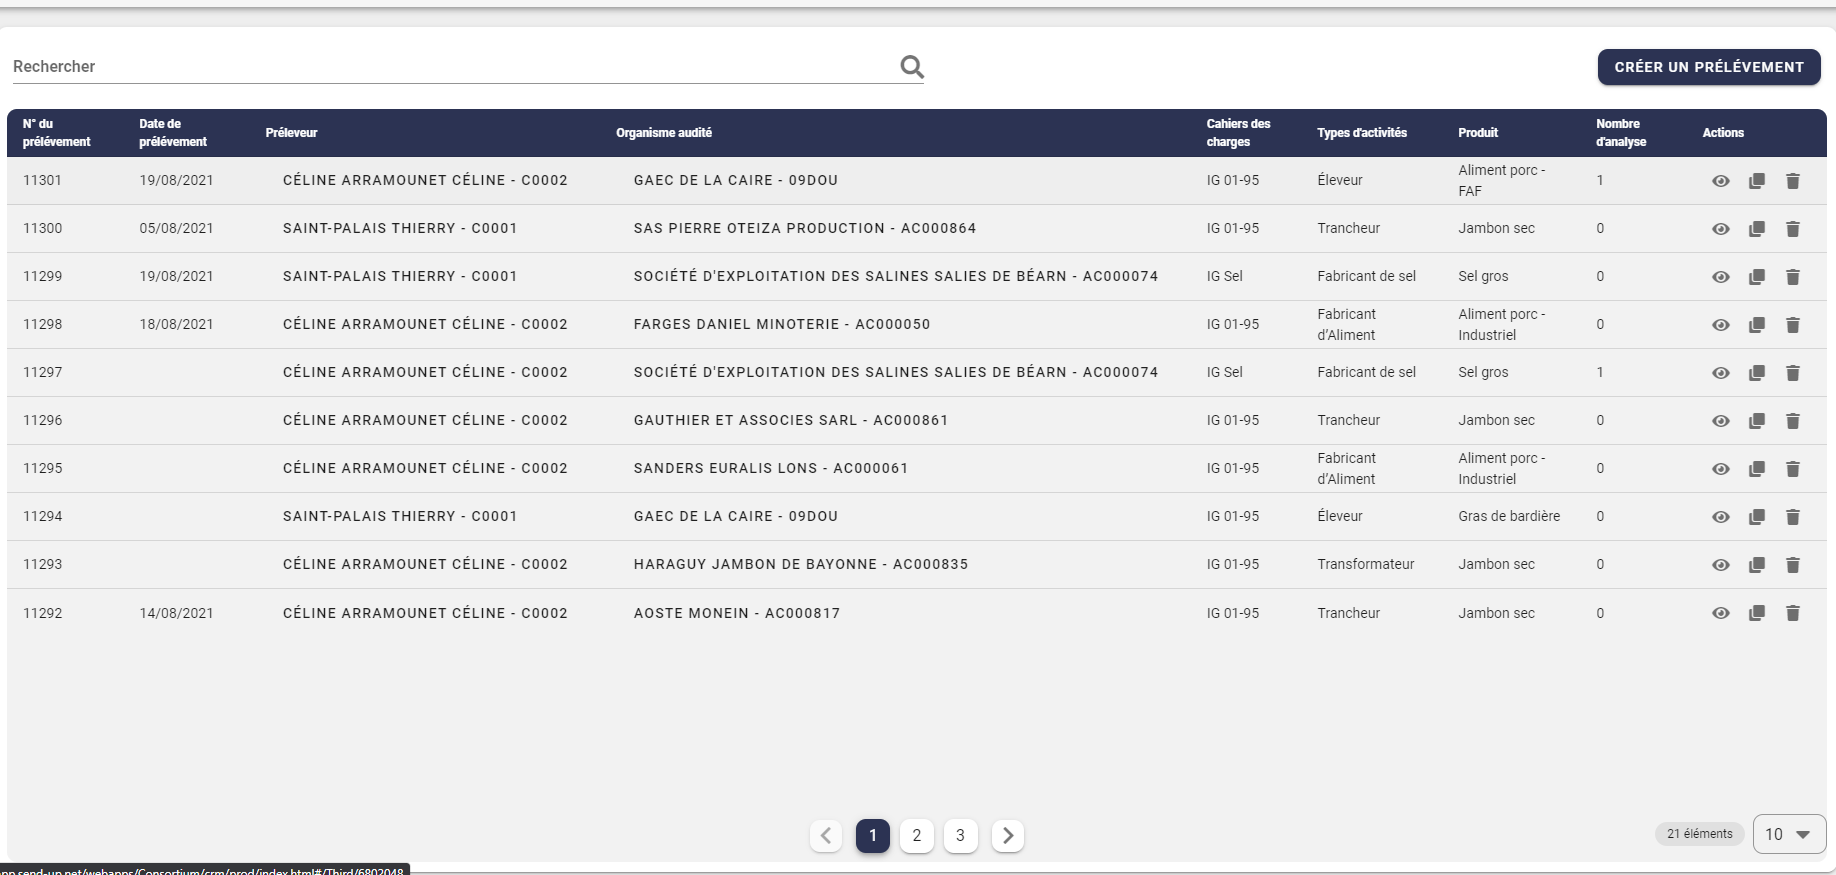
\includegraphics[width=\textwidth]{porcList.png}
    \caption{Listing des prélèvement}
    \label{fig:porcList}
\end{figure}

\begin{figure}[htbp]
    \center 
    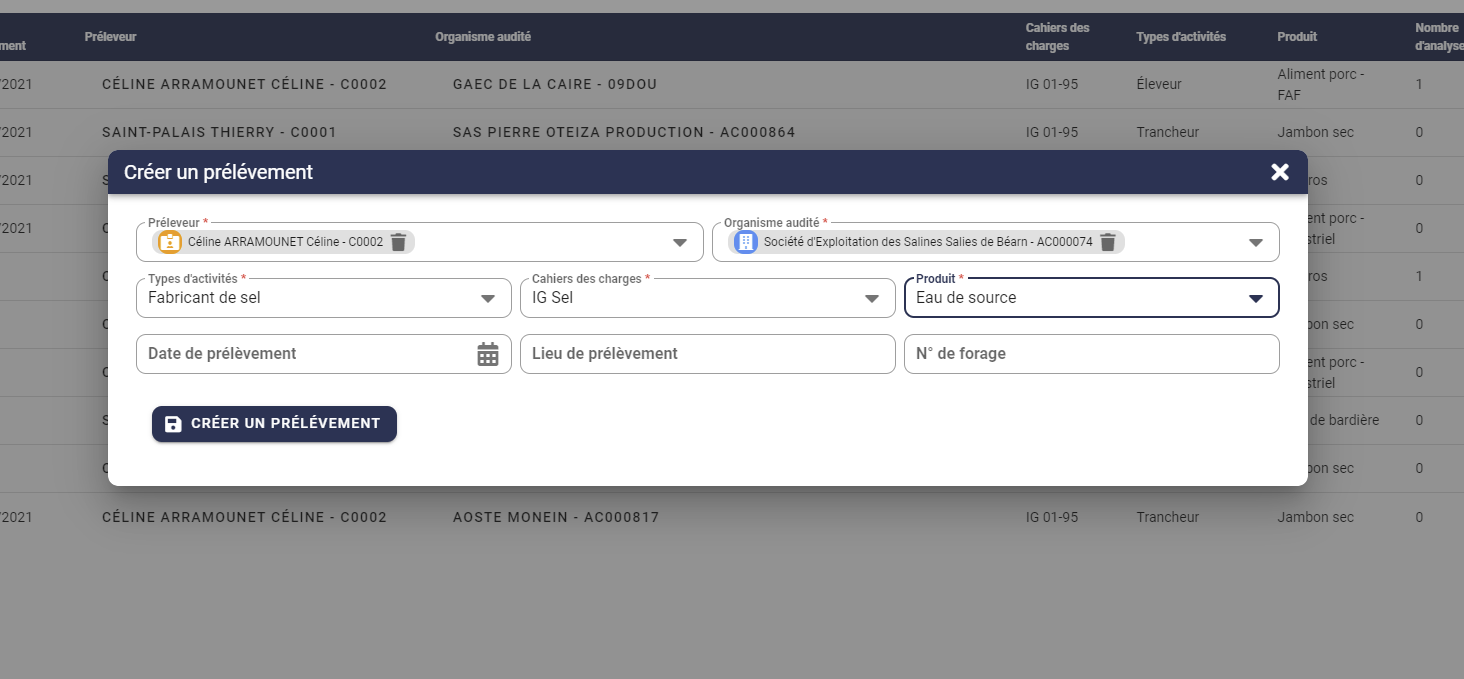
\includegraphics[width=\textwidth]{porcCreate.png}
    \caption{Création d'un prélèvement}
    \label{fig:porcCreate}
\end{figure}

\begin{figure}[htbp]
    \center 
    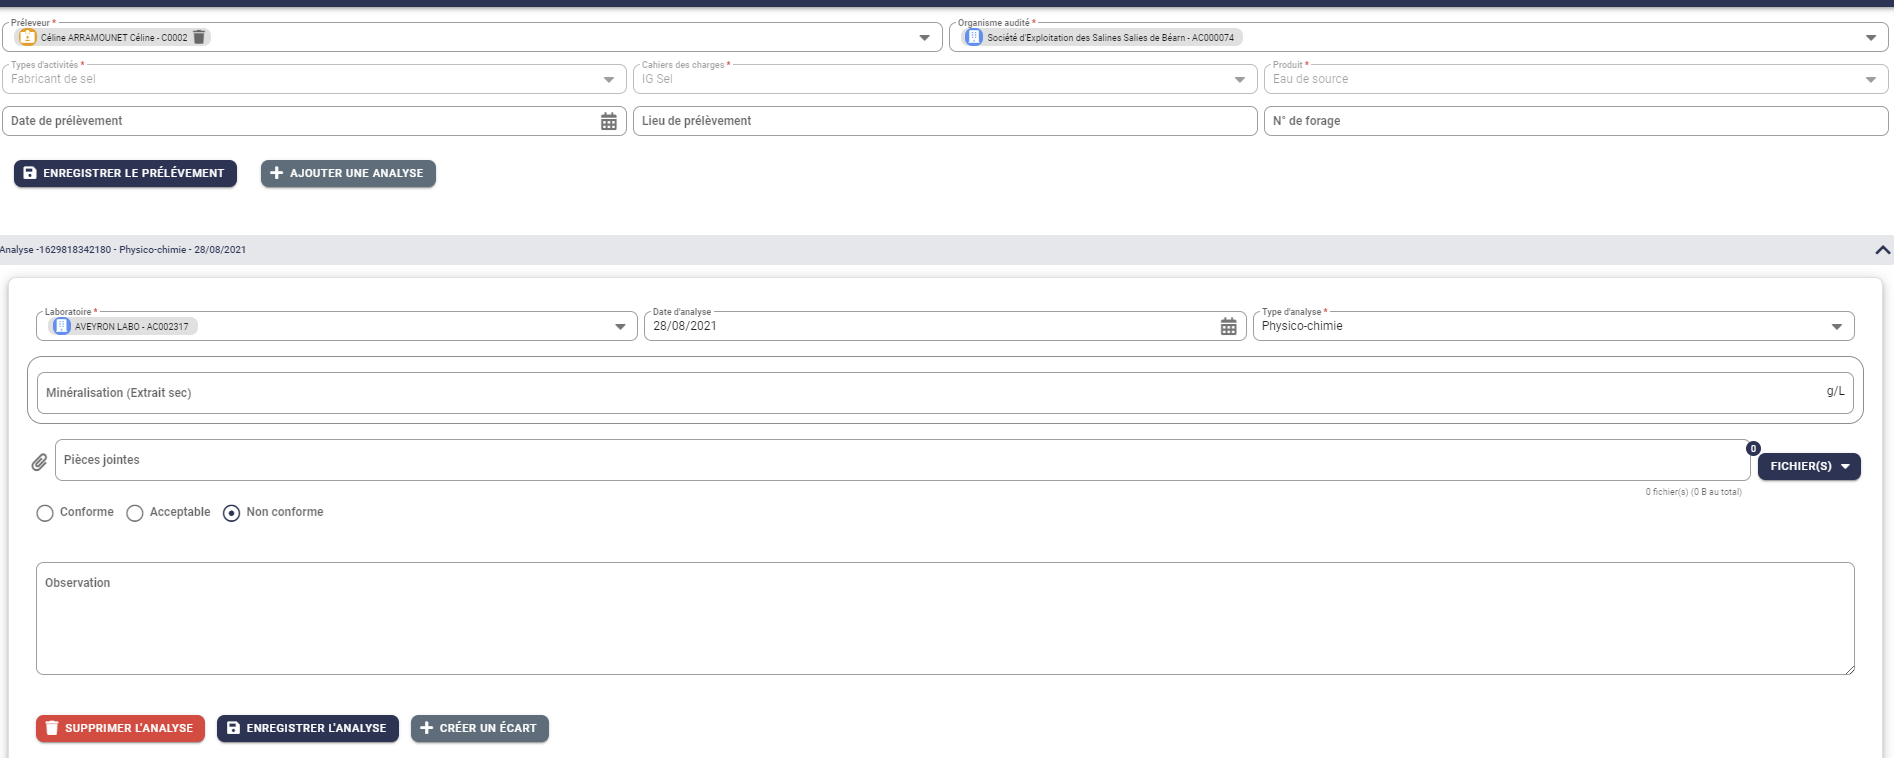
\includegraphics[width=\textwidth]{porcUpdate.png}
    \caption{Affichage d'un prélèvement et création d'une analyse}
    \label{fig:porcUpdate}
\end{figure}

\begin{figure}[htbp]
    \center 
    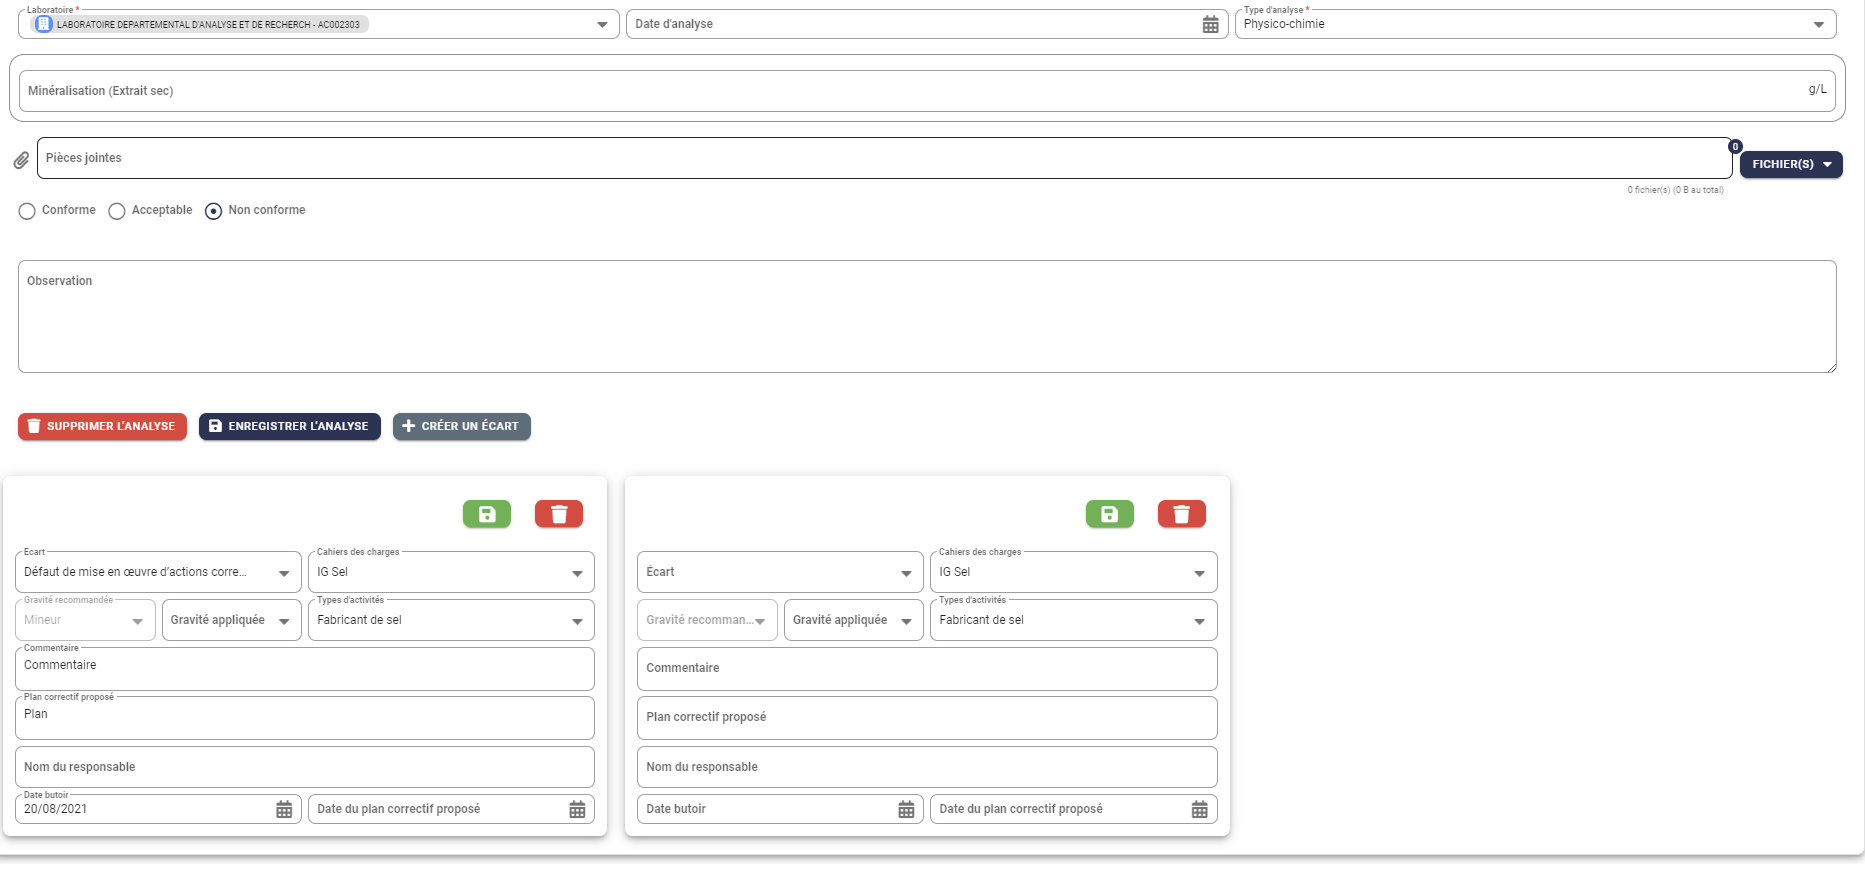
\includegraphics[width=\textwidth]{porcEcart.png}
    \caption{Créations de plusieurs écarts}
    \label{fig:porcEcart}
\end{figure}